\documentclass{article}

\usepackage[margin=1.2cm, top=1cm, bottom=1.8cm]{geometry}
\pagestyle{plain}
\linespread{1.4}

\usepackage{fontspec}
\usepackage{unicode-math}
\usepackage[main=greek, english]{babel}

\setmainfont{CMU Serif}
\setsansfont{CMU Sans Serif}
\setmonofont{CMU Typewriter Text}
\setmathfont{Latin Modern Math}

\usepackage{amsmath, enumitem}
\usepackage{dirtytalk, caption, subcaption, array, graphicx}
\usepackage{titlesec}
\usepackage{soul}
\usepackage[unicode]{hyperref}
\usepackage{verbatim}

\usepackage{pdfpages}

\usepackage{tikz}
\usetikzlibrary{arrows.meta, positioning}

\hypersetup{
    hidelinks,
    bookmarksopen=true,
    bookmarksnumbered=true,
    pdftitle={Συστήματα Αναμονής - 5η Εργαστηριακή Άσκηση},
    pdfauthor={Πέππας Μιχαήλ-Αθανάσιος}
}

\newcolumntype{P}[1]{>{\centering\arraybackslash}p{#1}}
\titleformat*{\subsubsection}{\large\bfseries}

\begin{document}

\begin{center}
    {
    \Large
    {
    \textbf{ΕΘΝΙΚΟ ΜΕΤΣΟΒΙΟ ΠΟΛΥΤΕΧΝΕΙΟ\\
    ΣΧΟΛΗ ΗΛΕΚΤΡΟΛΟΓΩΝ ΜΗΧΑΝΙΚΩΝ\\
    ΚΑΙ ΜΗΧΑΝΙΚΩΝ ΥΠΟΛΟΓΙΣΤΩΝ\\}
    }

    \vspace{1.5cm}
    \rule{18cm}{0.5pt}

    Τομέας Επικοινωνιών, Ηλεκτρονικής και Συστημάτων Πληροφορικής\\
    Εργαστήριο Διαχείρισης και Βέλτιστου Σχεδιασμού Δικτύων Τηλεματικής - NETMODE\\

    \rule{18cm}{0.5pt}

    \textbf{Συστήματα Αναμονής}\\
    \textbf{$\mathbf{5^{η}}$ Εργαστηριακή Άσκηση}\\
    }
\end{center}

\vspace{0.8cm}
\begin{center}
\includegraphics[width=7cm]{EMP Logo.png}
\end{center}

\Large
{
\vspace{0.8cm}
\noindent
\textbf{Στοιχεία Φοιτητή}
\begin{itemize}
    \item Όνομα: Πέππας Μιχαήλ-Αθανάσιος
    \item Αριθμός Μητρώου: 03121026
    \item $4^{\eta}$ Εργαστηριακή Ομάδα (Δευτέρα, 12:45-14:30)
    \item Ημερομηνία Διεξαγωγής Εργαστηρίου: 20.04.2026
    \item Ημερομηνία Παράδοσης Αναφοράς: 26.04.2026
\end{itemize}
}

\newpage
\tableofcontents

\newpage
\section{Προσομοίωση διακριτών γεγονότων Web Server}

\subsection{Περιγραφή και μοντελοποίηση του συστήματος}

Στο πρώτο μέρος της άσκησης μελετάμε μέσω προσομοίωσης διακριτών γεγονότων έναν Web Server, ο οποίος εξυπηρετεί αιτήματα με σειρά FIFO. Κάθε request που φτάνει στο σύστημα δημιουργεί αρχικά μία εργασία τύπου 1. Όταν ολοκληρωθεί η εργασία τύπου 1, το ίδιο request δεν αποχωρεί από το σύστημα, αλλά δημιουργεί μία εργασία τύπου 2, η οποία τοποθετείται ξανά στο τέλος της ίδιας ουράς. Το request θεωρείται πλήρως εξυπηρετημένο μόνο όταν ολοκληρωθεί και η εργασία τύπου 2.

Η βασική ιδιαιτερότητα του μοντέλου είναι ότι οι δύο φάσεις του ίδιου request δεν εξυπηρετούνται απαραίτητα διαδοχικά. Η δεύτερη φάση εισέρχεται ξανά στο τέλος της FIFO ουράς και μπορεί να προηγούνται άλλες εργασίες, είτε τύπου 1 είτε τύπου 2. Επομένως, το σύστημα είναι ένας single-server FIFO μηχανισμός με δύο φάσεις εξυπηρέτησης ανά request.

Οι αφίξεις ακολουθούν διαδικασία Poisson με ρυθμό $\lambda$ requests/sec. Συνεπώς, οι χρόνοι μεταξύ διαδοχικών αφίξεων είναι εκθετικά κατανεμημένοι. Επειδή η προσομοίωση υλοποιείται σε milliseconds, ο μέσος χρόνος μεταξύ αφίξεων είναι:
\[
    E[A] = \frac{1000}{\lambda} \text{ ms}.
\]

Οι χρόνοι εξυπηρέτησης των δύο τύπων εργασιών είναι ανεξάρτητοι και ακολουθούν διαφορετικές κατανομές:
\[
    S_1 \sim LogNormal(\mu=1,\sigma=1),
\]
και:
\[
    S_2 \sim Uniform(0.5,1).
\]
Για την εργασία τύπου 1, επειδή η λογαριθμοκανονική κατανομή προκύπτει ως $X=e^Y$, με $Y \sim N(\mu,\sigma^2)$, η μέση τιμή της είναι:
\[
    E[S_1] = e^{\mu + \sigma^2/2} = e^{1+1/2} = e^{1.5} \simeq 4.481689 \text{ ms}.
\]
Για την εργασία τύπου 2 έχουμε:
\[
    E[S_2] = \frac{0.5+1}{2} = 0.75 \text{ ms}.
\]
Άρα, το μέσο συνολικό service requirement ανά request είναι:
\[
    E[S] = E[S_1] + E[S_2] \simeq 5.231689 \text{ ms}.
\]

Η προσομοίωση είναι μη τερματική ως προς τη φύση του συστήματος, αλλά κάθε run σταματά τεχνητά όταν εξυπηρετηθούν πλήρως $10^4$ requests. Η βασική κατάσταση που διατηρεί ο προσομοιωτής περιλαμβάνει τον τρέχοντα χρόνο, την κατάσταση του server, τη FIFO ουρά, τους μετρητές αφίξεων και ολοκληρωμένων requests, καθώς και τα χρονικά logs που απαιτούνται για τον υπολογισμό των μέσων μεγεθών.

\subsection{Δομή της προσομοίωσης διακριτών γεγονότων}

Στην προσομοίωση διακριτών γεγονότων ο χρόνος δεν προχωρά με σταθερό βήμα, αλλά μετακινείται από γεγονός σε γεγονός. Στο συγκεκριμένο πρόβλημα υπάρχουν τρεις τύποι γεγονότων:
\begin{itemize}
    \item \textbf{ARRIVAL}: φτάνει νέο request και δημιουργείται εργασία τύπου 1.
    \item \textbf{DEPART1}: ολοκληρώνεται μία εργασία τύπου 1 και το ίδιο request δημιουργεί εργασία τύπου 2.
    \item \textbf{DEPART2}: ολοκληρώνεται μία εργασία τύπου 2 και το request αποχωρεί από το σύστημα.
\end{itemize}

Στο γεγονός ARRIVAL αυξάνεται ο μετρητής αφίξεων και προγραμματίζεται η επόμενη άφιξη. Αν ο server είναι ελεύθερος, η νέα εργασία τύπου 1 ξεκινά άμεσα εξυπηρέτηση. Διαφορετικά, τοποθετείται στο τέλος της ουράς.

Στο γεγονός DEPART1 καταγράφεται ο χρόνος απόκρισης της πρώτης φάσης και δημιουργείται νέα εργασία τύπου 2, η οποία προστίθεται στο τέλος της FIFO ουράς. Στη συνέχεια, ο server επιλέγει την επόμενη εργασία από την κεφαλή της ουράς.

Στο γεγονός DEPART2 καταγράφεται ο χρόνος απόκρισης της δεύτερης φάσης, αυξάνεται ο αριθμός των πλήρως εξυπηρετημένων requests και, αν υπάρχουν άλλες εργασίες στην ουρά, ξεκινά η επόμενη εξυπηρέτηση. Διαφορετικά, ο server γίνεται idle.

Επειδή το μέγεθος της ουράς μεταβάλλεται μόνο στις χρονικές στιγμές γεγονότων, οι μέσοι αριθμοί εργασιών στο σύστημα πρέπει να υπολογίζονται ως χρονικά σταθμισμένοι μέσοι όροι. Αν $Q(t)$ είναι βηματική συνάρτηση, τότε:
\[
    \overline{Q} =
    \frac{\sum_i Q(t_i)\Delta t_i}{\sum_i \Delta t_i},
    \qquad
    \Delta t_i = t_{i+1}-t_i.
\]
Ο απλός αριθμητικός μέσος των τιμών του $Q(t)$ στα event times δεν είναι σωστός, διότι τα γεγονότα δεν απέχουν ισοχρονικά μεταξύ τους.

\newpage
\subsection{Ερώτημα A.1: Εκτέλεση για λ = 100 requests/sec}

Στο πρώτο ερώτημα εκτελέσαμε την προσομοίωση για:
\[
    \lambda = 100 \text{ requests/sec},
\]
μέχρι να εξυπηρετηθούν πλήρως $10^4$ requests. Η εκτέλεση έδωσε τα ακόλουθα βασικά αριθμητικά αποτελέσματα:

\begin{verbatim}
A.1  lambda = 100 req/sec, 10000 fully served requests
  t_end = 100837.637255 ms = 100.837637 sec
  arrivals = 10002, fully served = 10000
  R1 = 10.579663 ms, R2 = 6.398254 ms, R = 16.977038 ms
  throughput: type-1 = 99.179238 jobs/sec, type-2 = 99.169321 jobs/sec
  time-weighted mean jobs: N1 = 1.049398, N2 = 0.634528, N = 1.683926
\end{verbatim}

Στο Σχήμα~\ref{fig:a1_arrivals_served} παρουσιάζονται οι αθροιστικοί αριθμοί αφίξεων και πλήρως εξυπηρετημένων requests ως προς τον χρόνο. Οι δύο καμπύλες είναι πρακτικά σχεδόν ταυτισμένες. Αυτό είναι αναμενόμενο, επειδή για $\lambda=100$ το σύστημα είναι στάσιμο και δεν συσσωρεύει απεριόριστα μεγάλο πλήθος εργασιών.

\begin{figure}[h!]
    \centering
    
\includegraphics[width=0.95\textwidth]{lab5_part1_1.png}
    \caption{Αθροιστικός αριθμός αφίξεων και πλήρως εξυπηρετημένων requests για $\lambda=100$ requests/sec.}
    \label{fig:a1_arrivals_served}
\end{figure}

Στο Σχήμα~\ref{fig:a1_jobs_types} φαίνεται η εξέλιξη του πλήθους εργασιών τύπου 1 και τύπου 2 στο σύστημα, όπου ως σύστημα θεωρούμε τόσο την ουρά όσο και την εργασία που ενδεχομένως εξυπηρετείται εκείνη τη στιγμή. Παρατηρούμε ότι και τα δύο μεγέθη παρουσιάζουν τυχαίες διακυμάνσεις, αλλά δεν εμφανίζουν αυξητική τάση ως προς τον χρόνο. Αυτό είναι ακόμη μία ένδειξη στάσιμης λειτουργίας.

\begin{figure}[h!]
    \centering
    
\includegraphics[width=0.95\textwidth]{lab5_part1_2.png}
    \caption{Αριθμός εργασιών τύπου 1 και τύπου 2 στο σύστημα για $\lambda=100$ requests/sec.}
    \label{fig:a1_jobs_types}
\end{figure}

Στο Σχήμα~\ref{fig:a1_response_throughput} παρουσιάζονται οι μέσοι χρόνοι απόκρισης ανά φάση και οι αντίστοιχοι ρυθμοί ολοκλήρωσης εργασιών ανά δευτερόλεπτο. Ο μέσος χρόνος απόκρισης της εργασίας τύπου 1 είναι μεγαλύτερος από αυτόν της εργασίας τύπου 2, κάτι που συμφωνεί με το γεγονός ότι η εργασία τύπου 1 έχει σημαντικά μεγαλύτερο μέσο χρόνο εξυπηρέτησης:
\[
    E[S_1] \simeq 4.481689 \text{ ms}
    \quad \text{έναντι} \quad
    E[S_2]=0.75 \text{ ms}.
\]
Επιπλέον, οι δύο ρυθμοί ολοκλήρωσης είναι σχεδόν ίσοι και κοντά στο $\lambda=100$, διότι κάθε πλήρως εξυπηρετημένο request αντιστοιχεί σε μία εργασία τύπου 1 και μία εργασία τύπου 2.

\begin{figure}[h!]
    \centering
    
\includegraphics[width=0.95\textwidth]{lab5_part1_3.png}
    \caption{Μέσοι χρόνοι απόκρισης ανά φάση και μέσος αριθμός ολοκληρωμένων εργασιών ανά δευτερόλεπτο.}
    \label{fig:a1_response_throughput}
\end{figure}

Αριθμητικά, πήραμε:
\[
    R_1 = 10.579663 \text{ ms},
    \qquad
    R_2 = 6.398254 \text{ ms},
\]
και:
\[
    R = 16.977038 \text{ ms}.
\]
Οι τιμές αυτές είναι μεγαλύτερες από τους καθαρούς μέσους χρόνους εξυπηρέτησης, επειδή περιλαμβάνουν τόσο εξυπηρέτηση όσο και αναμονή στην ουρά. Αυτό είναι ιδιαίτερα σημαντικό: το $R_i$ δεν είναι απλώς service time, αλλά response time της αντίστοιχης φάσης.

\newpage
\subsection{Ερώτημα A.2: Στασιμότητα για διαφορετικές τιμές του λ}

Στο δεύτερο ερώτημα εκτελέσαμε την προσομοίωση για:
\[
    \lambda \in \{50,100,150,200,250\} \text{ requests/sec}.
\]
Το αναλυτικό κριτήριο στασιμότητας προκύπτει από το συνολικό μέσο έργο που εισάγει κάθε request στον server. Κάθε request απαιτεί κατά μέσο όρο:
\[
    E[S_1]+E[S_2] = e^{1.5}+0.75 \simeq 5.231689 \text{ ms}.
\]
Άρα ο βαθμός φόρτου του single-server συστήματος είναι:
\[
    \rho =
    \frac{\lambda(E[S_1]+E[S_2])}{1000}.
\]
Για να είναι το σύστημα στάσιμο, πρέπει:
\[
    \rho < 1.
\]
Επομένως:
\[
    \lambda < \frac{1000}{E[S_1]+E[S_2]}
    =
    \frac{1000}{5.231689}
    \simeq 191.142858 \text{ requests/sec}.
\]

Η έξοδος του προγράμματος για το ερώτημα αυτό ήταν:

\begin{verbatim}
A.2  Stability bound
  lambda < 191.142858 req/sec
  lambda =  50: rho = 0.261584 -> stationary
  lambda = 100: rho = 0.523169 -> stationary
  lambda = 150: rho = 0.784753 -> stationary
  lambda = 200: rho = 1.046338 -> non-stationary
  lambda = 250: rho = 1.307922 -> non-stationary
\end{verbatim}

Άρα, αναλυτικά, οι τιμές:
\[
    \lambda = 50,100,150
\]
αντιστοιχούν σε στάσιμη λειτουργία, ενώ οι τιμές:
\[
    \lambda = 200,250
\]
αντιστοιχούν σε μη στάσιμη λειτουργία.

Στο Σχήμα~\ref{fig:a2_stationarity} φαίνεται το συνολικό πλήθος εργασιών στο σύστημα ως συνάρτηση του χρόνου για τις πέντε τιμές του $\lambda$. Για $\lambda=50,100,150$, το πλήθος εργασιών εμφανίζει διακυμάνσεις γύρω από κάποια πεπερασμένη περιοχή τιμών, χωρίς συστηματική ανοδική τάση. Αντίθετα, για $\lambda=200$ και κυρίως για $\lambda=250$, παρατηρούμε καθαρή συσσώρευση εργασιών, κάτι που συμφωνεί με το γεγονός ότι $\rho>1$.

\begin{figure}[h!]
    \centering
    
\includegraphics[width=0.95\textwidth, height=13cm]{lab5_part1_4.png}
    \caption{Συνολικό πλήθος εργασιών στο σύστημα για $\lambda \in \{50,100,150,200,250\}$ requests/sec.}
    \label{fig:a2_stationarity}
\end{figure}

Η συμπεριφορά αυτή συμφωνεί πλήρως με τη θεωρία. Όταν $\rho<1$, ο server μπορεί κατά μέσο όρο να επεξεργάζεται το εισερχόμενο έργο και η ουρά έχει στάσιμη κατανομή. Όταν $\rho \geq 1$, ο μέσος ρυθμός εισερχόμενου έργου είναι μεγαλύτερος ή ίσος από τη δυνατότητα εξυπηρέτησης του server, με αποτέλεσμα το σύστημα να μην έχει στάσιμη κατάσταση και η ουρά να αυξάνεται μακροπρόθεσμα.

\newpage
\subsection{Ερώτημα A.3: Διαστήματα εμπιστοσύνης και αφαίρεση μεταβατικής περιόδου}

Στο τρίτο ερώτημα εκτελέσαμε:
\[
    n=30
\]
ανεξάρτητες επαναλήψεις της προσομοίωσης για:
\[
    \lambda = 100
    \quad \text{και} \quad
    \lambda = 180
    \text{ requests/sec}.
\]
Κάθε επανάληψη δίνει έναν χρονικά σταθμισμένο μέσο αριθμό εργασιών τύπου 1 και τύπου 2 στο σύστημα. Τα $30$ αυτά ανεξάρτητα μεγέθη χρησιμοποιούνται για τον υπολογισμό διαστημάτων εμπιστοσύνης 95\%.

Η χρήση ανεξάρτητων επαναλήψεων είναι απαραίτητη, επειδή οι τιμές $Q(t)$ μέσα σε ένα μόνο simulation run δεν αποτελούν ανεξάρτητα δείγματα. Αν η ουρά έχει μία συγκεκριμένη τιμή σε κάποια στιγμή, είναι πολύ πιθανό να έχει κοντινή τιμή και αμέσως μετά. Άρα, για τα confidence intervals δεν χρησιμοποιούμε τις διαδοχικές τιμές της ουράς, αλλά έναν συνοπτικό μέσο όρο από κάθε ανεξάρτητη εκτέλεση.

Για το διάστημα εμπιστοσύνης της μέσης τιμής χρησιμοποιούμε:
\[
    \bar{x} \pm t_{n-1,1-\alpha/2}\frac{s}{\sqrt{n}},
    \qquad
    \alpha=0.05.
\]
Για τη διάμεσο χρησιμοποιούμε διάστημα βασισμένο σε στατιστικές τάξης:
\[
    [X_{(k)}, X_{(n+1-k)}],
\]
με:
\[
    k =
    \left\lfloor
    \frac{n}{2} - z_{1-\alpha/2}\frac{\sqrt{n}}{2}
    \right\rfloor.
\]

\subsubsection{Μέθοδος αφαίρεσης transient}

Επειδή η προσομοίωση ξεκινά από άδειο σύστημα, το αρχικό τμήμα δεν είναι απαραίτητα αντιπροσωπευτικό της μόνιμης κατάστασης. Για τον λόγο αυτό χρησιμοποιήσαμε τη μέθοδο MQS, δηλαδή το running time-weighted mean queue size:
\[
    MQS(t) = \frac{1}{t}\int_0^t Q(s)\,ds.
\]
Η βασική ιδέα είναι ότι το $MQS(t)$ αρχικά επηρεάζεται έντονα από την αρχική κατάσταση, αλλά στη συνέχεια τείνει να σταθεροποιείται γύρω από τη μέση τιμή μόνιμης λειτουργίας. Στην υλοποίηση επιλέχθηκε ως cutoff το πρώτο $30\%$ του χρόνου κάθε run, επιλογή που επιβεβαιώνεται και από τα MQS διαγράμματα.

Στο Σχήμα~\ref{fig:a3_mqs} παρουσιάζεται το $MQS(t)$ για $\lambda=100$ και $\lambda=180$. Για $\lambda=100$ παρατηρούμε ότι μετά τα πρώτα δευτερόλεπτα η καμπύλη σταθεροποιείται γρήγορα. Για $\lambda=180$, επειδή το σύστημα λειτουργεί κοντά στο όριο στασιμότητας, η καμπύλη εμφανίζει πολύ μεγαλύτερο transient και υψηλότερη μεταβλητότητα.

\begin{figure}[h!]
    \centering
    
\includegraphics[width=0.95\textwidth]{lab5_part1_5.png}
    \caption{MQS$(t)$ για $\lambda=100$ και $\lambda=180$ requests/sec και επιλογή cutoff στο 30\% του run time.}
    \label{fig:a3_mqs}
\end{figure}

Για $\lambda=180$ ο βαθμός φόρτου είναι:
\[
    \rho_{180}
    =
    \frac{180 \cdot 5.231689}{1000}
    \simeq 0.9417.
\]
Άρα το σύστημα είναι μεν στάσιμο, αλλά βρίσκεται πολύ κοντά στο όριο $\rho=1$. Αυτό εξηγεί γιατί τα confidence intervals είναι πολύ πλατύτερα σε σχέση με την περίπτωση $\lambda=100$.

\newpage
\subsubsection{Αποτελέσματα διαστημάτων εμπιστοσύνης}

Η έξοδος του προγράμματος για τα confidence intervals ήταν:

\begin{verbatim}
A.3  95% confidence intervals, n = 30 replications
  Transient removal rule: remove first 30% of each run, guided by MQS(t) plots.

  lambda = 100 req/sec
    Full trace:
      type 1: mean CI [1.014991, 1.056171], median CI [1.011125, 1.063644]
      type 2: mean CI [0.603187, 0.632896], median CI [0.601051, 0.631790]
    After transient removal:
      type 1: mean CI [1.008903, 1.060815], median CI [0.984703, 1.060240]
      type 2: mean CI [0.599920, 0.636938], median CI [0.586471, 0.647216]

  lambda = 180 req/sec
    Full trace:
      type 1: mean CI [14.476681, 18.489433], median CI [13.566229, 18.068241]
      type 2: mean CI [13.679712, 17.688760], median CI [12.826022, 17.198553]
    After transient removal:
      type 1: mean CI [14.638395, 19.446088], median CI [13.488622, 18.944785]
      type 2: mean CI [13.891899, 18.707440], median CI [12.648005, 18.337582]
\end{verbatim}

Για $\lambda=100$, τα διαστήματα εμπιστοσύνης είναι σχετικά στενά. Αυτό είναι αναμενόμενο, επειδή το σύστημα έχει μέτριο φορτίο:
\[
    \rho_{100} \simeq 0.5232.
\]
Άρα οι διακυμάνσεις του πλήθους εργασιών είναι περιορισμένες και οι ανεξάρτητες επαναλήψεις παράγουν σχετικά κοντινές εκτιμήσεις.

Για $\lambda=180$, τα διαστήματα εμπιστοσύνης είναι πολύ πλατύτερα. Αυτό συμβαίνει επειδή το σύστημα βρίσκεται κοντά στο όριο αστάθειας. Σε τέτοιες περιπτώσεις, μικρές τυχαίες αποκλίσεις στην ακολουθία αφίξεων και εξυπηρετήσεων μπορούν να οδηγήσουν σε μεγάλες παροδικές ουρές, άρα οι εκτιμήσεις από run σε run διαφέρουν περισσότερο.

Η αφαίρεση του transient δεν αλλάζει δραματικά τα κέντρα των διαστημάτων, αλλά μεταβάλλει ελαφρώς τόσο τα άκρα όσο και το πλάτος τους. Για $\lambda=100$ η επίδραση είναι μικρή, επειδή το σύστημα φτάνει γρήγορα σε στάσιμη λειτουργία. Για $\lambda=180$ η επίδραση είναι πιο αισθητή, επειδή η αρχική περίοδος και η αργότερη σύγκλιση της ουράς έχουν μεγαλύτερο ρόλο.

Συνολικά, τα αποτελέσματα επιβεβαιώνουν ότι όσο πιο κοντά βρίσκεται το σύστημα στο $\rho=1$, τόσο περισσότερες επαναλήψεις ή/και μεγαλύτερη διάρκεια προσομοίωσης απαιτούνται για πιο στενά και αξιόπιστα confidence intervals.

\newpage
\subsection{Ερώτημα A.4: Επαλήθευση του νόμου Little}

Στο τέταρτο ερώτημα επαληθεύουμε τον νόμο του Little:
\[
    N = \lambda R.
\]
Στη συγκεκριμένη προσομοίωση το $R$ είναι ο μέσος end-to-end χρόνος απόκρισης ενός request, δηλαδή από την άφιξή του μέχρι την ολοκλήρωση της δεύτερης φάσης. Επομένως:
\[
    R = R_1 + R_2.
\]
Το $N$ είναι ο χρονικά σταθμισμένος μέσος αριθμός εργασιών στο σύστημα:
\[
    N =
    \overline{Q_1 + Q_2}.
\]
Χρειάζεται ιδιαίτερη προσοχή στις μονάδες. Το $\lambda$ δίνεται σε requests/sec, ενώ το $R$ έχει υπολογιστεί σε milliseconds. Άρα χρησιμοποιούμε:
\[
    \lambda_{ms} = \frac{\lambda}{1000}.
\]

Η έξοδος του προγράμματος για τον νόμο Little ήταν:

\begin{verbatim}
A.4  Little's Law, lambda = 100 req/sec
  Without transient removal:
    R = 16.977038 ms, N_sim = 1.683926, lambda*R = 1.697704, error = 0.818167 %
  With transient removal:
    R = 16.830559 ms, N_sim = 1.651705, lambda*R = 1.683056, error = 1.898066 %
\end{verbatim}

Χωρίς αφαίρεση transient έχουμε:
\[
    R = 16.977038 \text{ ms},
\]
και:
\[
    \lambda_{ms}R
    =
    0.1 \cdot 16.977038
    =
    1.697704.
\]
Η προσομοίωση δίνει:
\[
    N_{\text{sim}} = 1.683926.
\]
Το σχετικό σφάλμα είναι:
\[
    0.818167\%.
\]
Άρα ο νόμος Little επαληθεύεται με πολύ καλή ακρίβεια.

Μετά την αφαίρεση του transient, έχουμε:
\[
    R = 16.830559 \text{ ms},
\]
και:
\[
    \lambda_{ms}R = 1.683056.
\]
Το αντίστοιχο χρονικά σταθμισμένο μέσο πλήθος εργασιών είναι:
\[
    N_{\text{sim}} = 1.651705,
\]
με σχετικό σφάλμα:
\[
    1.898066\%.
\]

Το γεγονός ότι το σφάλμα μετά την αφαίρεση transient είναι λίγο μεγαλύτερο δεν αποτελεί πρόβλημα. Ο νόμος Little ισχύει ακριβώς στη μόνιμη κατάσταση και στο όριο μεγάλου χρόνου, ενώ εδώ χρησιμοποιείται ένα πεπερασμένο single-run δείγμα και ένα συγκεκριμένο cutoff. Επιπλέον, μετά το cutoff χρησιμοποιούνται λιγότερες παρατηρήσεις, άρα είναι φυσιολογικό να εμφανιστεί ελαφρώς μεγαλύτερη δειγματική απόκλιση.

Το σημαντικό συμπέρασμα είναι ότι και στις δύο περιπτώσεις το σφάλμα είναι μικρό, κάτω από 2\%, γεγονός που επιβεβαιώνει ότι η προσομοίωση είναι συνεπής με τη βασική θεωρία των συστημάτων αναμονής.

\subsection{Συνολικό συμπέρασμα πρώτου μέρους}

Τα αποτελέσματα του πρώτου μέρους είναι συνεπή τόσο με τη θεωρία όσο και με τη φυσική ερμηνεία του συστήματος.

Αρχικά, για $\lambda=100$ requests/sec, το σύστημα λειτουργεί σε σαφώς στάσιμη περιοχή, αφού:
\[
    \rho = 0.523169 < 1.
\]
Αυτό φαίνεται άμεσα από την σχεδόν πλήρη ταύτιση των αθροιστικών αφίξεων και εξυπηρετήσεων, καθώς και από το ότι οι καμπύλες των εργασιών τύπου 1 και τύπου 2 δεν εμφανίζουν ανοδική μακροχρόνια τάση. Ο μέσος end-to-end χρόνος απόκρισης είναι περίπου $16.98$ ms, ενώ ο χρονικά σταθμισμένος μέσος αριθμός εργασιών στο σύστημα είναι περίπου $1.68$.

Στη συνέχεια, η ανάλυση της στασιμότητας δείχνει ότι το κρίσιμο όριο είναι:
\[
    \lambda_{\max} \simeq 191.142858 \text{ requests/sec}.
\]
Άρα οι τιμές $\lambda=50,100,150$ είναι στάσιμες, ενώ οι τιμές $\lambda=200,250$ δεν είναι στάσιμες. Τα αντίστοιχα διαγράμματα επιβεβαιώνουν πλήρως το αναλυτικό αποτέλεσμα: στα στάσιμα σενάρια η ουρά παραμένει σε πεπερασμένες διακυμάνσεις, ενώ στα μη στάσιμα εμφανίζει αυξητική τάση.

Τα confidence intervals δείχνουν επίσης την αναμενόμενη εξάρτηση από το φορτίο. Για $\lambda=100$ είναι στενά, ενώ για $\lambda=180$ γίνονται πολύ πλατύτερα, επειδή το σύστημα βρίσκεται κοντά στο όριο $\rho=1$. Αυτό είναι ένα κλασικό χαρακτηριστικό των ουρών: όσο το φορτίο πλησιάζει τη μονάδα, τόσο αυξάνεται η μεταβλητότητα, οι ουρές γίνονται πιο έντονες και η προσομοίωση χρειάζεται περισσότερες παρατηρήσεις για σταθερές εκτιμήσεις.

Η μέθοδος MQS αποτελεί εύλογο εργαλείο για την επιλογή transient cutoff. Τα διαγράμματα δείχνουν ότι για $\lambda=100$ το running time-weighted average σταθεροποιείται γρήγορα, ενώ για $\lambda=180$ η σταθεροποίηση είναι πιο αργή και η καμπύλη πιο ευμετάβλητη. Η επιλογή αποκοπής του πρώτου 30\% του run είναι επομένως συντηρητική και κατάλληλη για την παρούσα άσκηση.

Τέλος, ο νόμος του Little επαληθεύεται με μικρό σφάλμα τόσο πριν όσο και μετά την αφαίρεση transient. Αυτό λειτουργεί ως επιπλέον έλεγχος ορθότητας, επειδή συνδέει τρεις ποσότητες που υπολογίζονται με διαφορετικό τρόπο: τον ρυθμό αφίξεων, τον μέσο χρόνο απόκρισης και τον χρονικά σταθμισμένο μέσο αριθμό εργασιών στο σύστημα.

Συνολικά, μπορούμε να συμπεράνουμε ότι η προσομοίωση είναι σωστή. Τα διαγράμματα συμφωνούν με τα αναλυτικά κριτήρια στασιμότητας, τα confidence intervals έχουν λογική συμπεριφορά, και ο νόμος Little επιβεβαιώνεται με μικρή απόκλιση.

\newpage
\section{Ανοιχτό δίκτυο ουρών αναμονής}

\subsection{Περιγραφή του δικτύου και παραδοχές Jackson}

Στο δεύτερο μέρος της άσκησης μελετάμε ένα ανοιχτό δίκτυο ουρών αναμονής με πέντε ουρές:
\[
    Q_1,Q_2,Q_3,Q_4,Q_5.
\]
Οι εξωτερικές αφίξεις εισέρχονται στο δίκτυο με ρυθμούς $\lambda_1$ και $\lambda_2$, ενώ κάθε ουρά $Q_i$ διαθέτει έναν εξυπηρετητή με εκθετικά κατανεμημένους χρόνους εξυπηρέτησης και ρυθμό $\mu_i$.

Για να μπορεί το δίκτυο να μελετηθεί ως ανοιχτό δίκτυο Jackson, πρέπει να ισχύουν οι βασικές παραδοχές:
\begin{itemize}
    \item οι εξωτερικές αφίξεις είναι Poisson,
    \item οι χρόνοι εξυπηρέτησης σε κάθε ουρά είναι εκθετικά κατανεμημένοι,
    \item οι εξυπηρετήσεις είναι ανεξάρτητες μεταξύ τους και ανεξάρτητες από τις αφίξεις,
    \item μετά από κάθε εξυπηρέτηση, ο πελάτης δρομολογείται με σταθερές πιθανότητες σε επόμενη ουρά ή αποχωρεί από το δίκτυο,
    \item οι πιθανότητες δρομολόγησης δεν εξαρτώνται από την κατάσταση του δικτύου,
    \item κάθε ουρά έχει άπειρη χωρητικότητα,
    \item κάθε κόμβος μπορεί να θεωρηθεί ως ξεχωριστό σύστημα $M/M/1$ με δικό του συνολικό ρυθμό άφιξης,
    \item το δίκτυο είναι εργοδικό, δηλαδή για κάθε ουρά ισχύει $\rho_i<1$.
\end{itemize}

Το θεώρημα Jackson επιτρέπει, υπό τις παραπάνω παραδοχές, τη μελέτη του δικτύου ως γινόμενο ανεξάρτητων ουρών $M/M/1$. Συνεπώς, αφού βρούμε τους συνολικούς ρυθμούς άφιξης $\Gamma_i$ σε κάθε κόμβο, μπορούμε να υπολογίσουμε:
\[
    \rho_i = \frac{\Gamma_i}{\mu_i},
    \qquad
    E[N_i] = \frac{\rho_i}{1-\rho_i}.
\]

\subsection{Μεταβάσεις και πιθανότητες δρομολόγησης}

Από το σχήμα του δικτύου προκύπτουν οι εξής δρομολογήσεις:

\[
\begin{array}{c|c|c}
\text{Από} & \text{Προς} & \text{Πιθανότητα} \\
\hline
Q_1 & Q_2 & \frac{1}{2} \\
Q_1 & Q_3 & \frac{1}{4} \\
Q_1 & \text{Έξοδος} & \frac{1}{4} \\
Q_2 & Q_3 & \frac{1}{3} \\
Q_2 & Q_4 & \frac{2}{3} \\
Q_3 & Q_5 & 1 \\
Q_4 & Q_5 & \frac{3}{5} \\
Q_4 & \text{Έξοδος} & \frac{2}{5} \\
Q_5 & \text{Έξοδος} & 1
\end{array}
\]

Οι πιθανότητες $Q_1 \to Q_3$ και $Q_2 \to Q_4$ προκύπτουν ως συμπληρωματικές πιθανότητες των αντίστοιχων διακλαδώσεων. Συγκεκριμένα:
\[
    P(Q_1 \to Q_3) = 1-\frac{1}{2}-\frac{1}{4} = \frac{1}{4},
\]
και:
\[
    P(Q_2 \to Q_4) = 1-\frac{1}{3} = \frac{2}{3}.
\]

Για πληρότητα, στο Σχήμα~\ref{fig:jackson_network} δίνεται σχηματική αναπαράσταση του δικτύου με τις βασικές πιθανότητες δρομολόγησης.

\begin{figure}[h!]
\centering
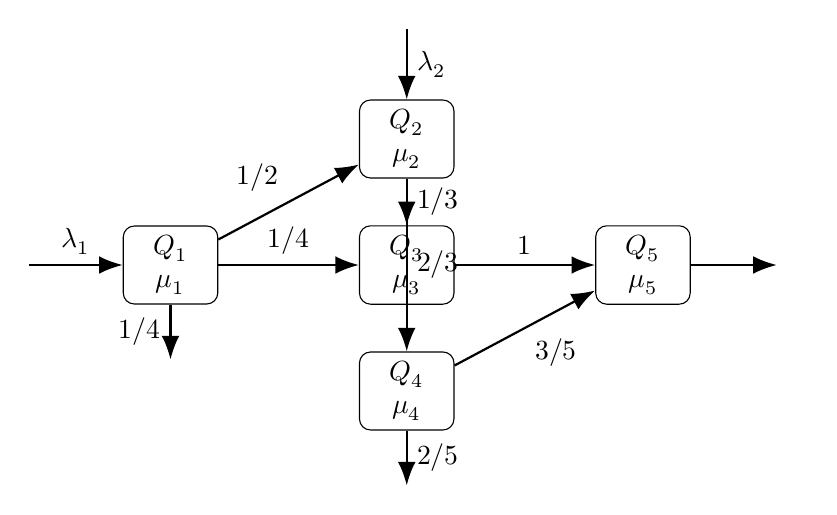
\begin{tikzpicture}[
    queue/.style={draw, rounded corners, minimum width=1.2cm, minimum height=0.8cm, align=center},
    arr/.style={-{Latex[length=3mm]}, thick},
    node distance=2.2cm
]
    \node[queue] (q1) at (0,0) {$Q_1$\\$\mu_1$};
    \node[queue] (q2) at (3,1.6) {$Q_2$\\$\mu_2$};
    \node[queue] (q3) at (3,0) {$Q_3$\\$\mu_3$};
    \node[queue] (q4) at (3,-1.6) {$Q_4$\\$\mu_4$};
    \node[queue] (q5) at (6,0) {$Q_5$\\$\mu_5$};

    \draw[arr] (-1.8,0) -- node[above] {$\lambda_1$} (q1);
    \draw[arr] (3,3.0) -- node[right] {$\lambda_2$} (q2);

    \draw[arr] (q1) -- node[above left] {$1/2$} (q2);
    \draw[arr] (q1) -- node[above] {$1/4$} (q3);
    \draw[arr] (q1) -- ++(0,-1.2) node[midway,left] {$1/4$};

    \draw[arr] (q2) -- node[right] {$1/3$} (q3);
    \draw[arr] (q2) -- node[right] {$2/3$} (q4);

    \draw[arr] (q3) -- node[above] {$1$} (q5);

    \draw[arr] (q4) -- node[below right] {$3/5$} (q5);
    \draw[arr] (q4) -- ++(0,-1.2) node[midway,right] {$2/5$};

    \draw[arr] (q5) -- ++(1.7,0) node[above] {Έξοδος};
\end{tikzpicture}
\caption{Σχηματική αναπαράσταση του ανοιχτού δικτύου ουρών Jackson.}
\label{fig:jackson_network}
\end{figure}

\subsection{Ερώτημα Β.2: Εξισώσεις ροής και εντάσεις φορτίου}

Για την εφαρμογή του θεωρήματος Jackson πρέπει πρώτα να βρούμε τον συνολικό ρυθμό άφιξης σε κάθε ουρά. Συμβολίζουμε αυτούς τους ρυθμούς με $\Gamma_i$, ώστε να μη συγχέονται με τους εξωτερικούς ρυθμούς $\lambda_1$ και $\lambda_2$.

Από τις δρομολογήσεις του σχήματος έχουμε:
\[
    \Gamma_1 = \lambda_1,
\]
\[
    \Gamma_2 = \lambda_2 + \frac{1}{2}\Gamma_1,
\]
\[
    \Gamma_3 = \frac{1}{4}\Gamma_1 + \frac{1}{3}\Gamma_2,
\]
\[
    \Gamma_4 = \frac{2}{3}\Gamma_2,
\]
\[
    \Gamma_5 = \Gamma_3 + \frac{3}{5}\Gamma_4.
\]

Αν αντικαταστήσουμε διαδοχικά, παίρνουμε όλες τις $\Gamma_i$ ως συναρτήσεις μόνο των εξωτερικών ρυθμών $\lambda_1,\lambda_2$:
\[
    \Gamma_1 = \lambda_1,
\]
\[
    \Gamma_2 = \lambda_2 + \frac{1}{2}\lambda_1,
\]
\[
    \Gamma_3 =
    \frac{1}{4}\lambda_1
    +
    \frac{1}{3}\left(\lambda_2+\frac{1}{2}\lambda_1\right)
    =
    \frac{5}{12}\lambda_1 + \frac{1}{3}\lambda_2,
\]
\[
    \Gamma_4 =
    \frac{2}{3}\left(\lambda_2+\frac{1}{2}\lambda_1\right)
    =
    \frac{1}{3}\lambda_1 + \frac{2}{3}\lambda_2,
\]
και:
\[
\begin{aligned}
    \Gamma_5
    &=
    \Gamma_3 + \frac{3}{5}\Gamma_4 \\
    &=
    \left(\frac{5}{12}\lambda_1+\frac{1}{3}\lambda_2\right)
    +
    \frac{3}{5}\left(\frac{1}{3}\lambda_1+\frac{2}{3}\lambda_2\right) \\
    &=
    \frac{37}{60}\lambda_1 + \frac{11}{15}\lambda_2.
\end{aligned}
\]

Επομένως, οι εντάσεις φορτίου των πέντε ουρών είναι:
\[
    \rho_1 = \frac{\lambda_1}{\mu_1},
\]
\[
    \rho_2 =
    \frac{\lambda_2+\frac{1}{2}\lambda_1}{\mu_2},
\]
\[
    \rho_3 =
    \frac{\frac{5}{12}\lambda_1+\frac{1}{3}\lambda_2}{\mu_3},
\]
\[
    \rho_4 =
    \frac{\frac{1}{3}\lambda_1+\frac{2}{3}\lambda_2}{\mu_4},
\]
\[
    \rho_5 =
    \frac{\frac{37}{60}\lambda_1+\frac{11}{15}\lambda_2}{\mu_5}.
\]

Η συνθήκη εργοδικότητας του δικτύου είναι:
\[
    \rho_i < 1,
    \qquad i=1,\ldots,5.
\]
Αν έστω μία ουρά έχει $\rho_i \geq 1$, τότε το δίκτυο δεν είναι εργοδικό.

Η συνάρτηση \texttt{intensities} που υλοποιήθηκε στο Octave υπολογίζει ακριβώς αυτές τις τιμές και επιστρέφει επίσης μία δυαδική ένδειξη εργοδικότητας.

\subsection{Ερώτημα Β.3: Μέσος αριθμός πελατών σε κάθε ουρά}

Κάθε ουρά του δικτύου, υπό τις παραδοχές Jackson, μπορεί να μελετηθεί ως ξεχωριστή ουρά $M/M/1$ με συνολικό ρυθμό άφιξης $\Gamma_i$ και ρυθμό εξυπηρέτησης $\mu_i$. Για μία ουρά $M/M/1$, όταν $\rho_i<1$, ο μέσος αριθμός πελατών στο σύστημα είναι:
\[
    E[N_i] = \frac{\rho_i}{1-\rho_i}.
\]

Άρα, αφού υπολογιστούν οι εντάσεις φορτίου $\rho_i$, οι μέσοι αριθμοί πελατών υπολογίζονται άμεσα από τον παραπάνω τύπο. Η συνάρτηση \texttt{mean\_clients} καλεί πρώτα την \texttt{intensities}, ελέγχει την εργοδικότητα, και στη συνέχεια επιστρέφει το διάνυσμα:
\[
    [E[N_1],E[N_2],E[N_3],E[N_4],E[N_5]].
\]

\subsection{Ερώτημα Β.4: Αριθμητική εφαρμογή για τις δοθείσες παραμέτρους}

Για το αριθμητικό ερώτημα της εκφώνησης δίνονται:
\[
    \lambda_1=10,
    \qquad
    \lambda_2=6,
\]
και:
\[
    \mu_1=15,\quad
    \mu_2=20,\quad
    \mu_3=10,\quad
    \mu_4=14,\quad
    \mu_5=12.
\]
Όλοι οι ρυθμοί είναι σε πελάτες ανά δευτερόλεπτο.

Η εκτέλεση του Octave έδωσε τους παρακάτω effective arrival rates:
\[
    \Gamma =
    [10,\ 11,\ 6.1666666667,\ 7.3333333333,\ 10.5666666667].
\]
Οι αντίστοιχες εντάσεις φορτίου είναι:
\[
    \rho =
    [0.6666666667,\ 0.55,\ 0.6166666667,\ 0.5238095238,\ 0.8805555556].
\]
Εφόσον όλες οι τιμές είναι μικρότερες της μονάδας, το δίκτυο είναι εργοδικό.

Οι μέσοι αριθμοί πελατών στις ουρές είναι:
\[
    E[N_i] =
    [2.0000000000,\ 1.2222222222,\ 1.6086956522,\ 1.1000000000,\ 7.3720930233].
\]
Άρα ο συνολικός μέσος αριθμός πελατών στο δίκτυο είναι:
\[
\begin{aligned}
    E[N]
    &=
    \sum_{i=1}^{5} E[N_i] \\
    &=
    13.3030108977.
\end{aligned}
\]

Ο συνολικός εξωτερικός ρυθμός εισόδου στο δίκτυο είναι:
\[
    \gamma = \lambda_1+\lambda_2 = 16 \text{ πελάτες/sec}.
\]
Επομένως, από τον νόμο του Little, ο μέσος end-to-end χρόνος καθυστέρησης ενός πελάτη στο δίκτυο είναι:
\[
    E[T] = \frac{E[N]}{\gamma}
    =
    \frac{13.3030108977}{16}
    =
    0.8314381811 \text{ sec}.
\]

Η έξοδος του προγράμματος για τα ερωτήματα Β.2--Β.4 ήταν:

\begin{verbatim}
Effective arrival rates Gamma_i:
  Gamma1 = 10.0000000000 clients/sec
  Gamma2 = 11.0000000000 clients/sec
  Gamma3 = 6.1666666667 clients/sec
  Gamma4 = 7.3333333333 clients/sec
  Gamma5 = 10.5666666667 clients/sec

Traffic intensities rho_i = Gamma_i / mu_i:
  rho1 = 0.6666666667
  rho2 = 0.5500000000
  rho3 = 0.6166666667
  rho4 = 0.5238095238
  rho5 = 0.8805555556

Ergodicity flag: 1
The network is ergodic because all rho_i are smaller than 1.

Mean clients E[N_i] in each queue:
  E[N1] = 2.0000000000
  E[N2] = 1.2222222222
  E[N3] = 1.6086956522
  E[N4] = 1.1000000000
  E[N5] = 7.3720930233

Total mean number of clients in the network:
  E[N] = sum_i E[N_i] = 13.3030108977

End-to-end mean delay by Little's Law:
  E[T] = E[N] / gamma_external = 0.8314381811 seconds
\end{verbatim}

Παρατηρούμε ότι η μεγαλύτερη συνεισφορά στον συνολικό αριθμό πελατών προέρχεται από την ουρά $Q_5$, όπου:
\[
    E[N_5] = 7.3720930233.
\]
Αυτό είναι αναμενόμενο, επειδή η $Q_5$ έχει και τη μεγαλύτερη ένταση φορτίου:
\[
    \rho_5 = 0.8805555556.
\]
Όσο το $\rho_i$ πλησιάζει τη μονάδα, ο όρος $\rho_i/(1-\rho_i)$ αυξάνεται απότομα. Επομένως, η $Q_5$ επηρεάζει δυσανάλογα τη συνολική καθυστέρηση του δικτύου.

\subsection{Ερώτημα Β.5: Στενωπός και μέγιστη τιμή του λ}

Η στενωπός του δικτύου είναι η ουρά με τη μεγαλύτερη ένταση φορτίου $\rho_i$. Για τις δοθείσες τιμές, έχουμε:
\[
    \max_i \rho_i = \rho_5 = 0.8805555556.
\]
Άρα η στενωπός του δικτύου είναι:
\[
    Q_5.
\]

Στη συνέχεια ζητείται η μέγιστη τιμή της παραμέτρου $\lambda_1$, ώστε το σύστημα να παραμένει εργοδικό, με σταθερό:
\[
    \lambda_2 = 6.
\]
Για να είναι το δίκτυο εργοδικό πρέπει να ισχύει:
\[
    \Gamma_i < \mu_i,
    \qquad i=1,\ldots,5.
\]

Από κάθε ουρά προκύπτει ένα άνω φράγμα για το $\lambda_1$.

Για την $Q_1$:
\[
    \Gamma_1 = \lambda_1 < \mu_1 = 15
    \Rightarrow
    \lambda_1 < 15.
\]

Για την $Q_2$:
\[
    \Gamma_2 = 6 + \frac{1}{2}\lambda_1 < 20
    \Rightarrow
    \lambda_1 < 28.
\]

Για την $Q_3$:
\[
    \Gamma_3 =
    \frac{5}{12}\lambda_1+\frac{1}{3}\cdot 6
    =
    \frac{5}{12}\lambda_1+2
    <10,
\]
άρα:
\[
    \frac{5}{12}\lambda_1 < 8
    \Rightarrow
    \lambda_1 < 19.2.
\]

Για την $Q_4$:
\[
    \Gamma_4 =
    \frac{1}{3}\lambda_1+\frac{2}{3}\cdot 6
    =
    \frac{1}{3}\lambda_1+4
    <14,
\]
άρα:
\[
    \lambda_1 < 30.
\]

Για την $Q_5$:
\[
    \Gamma_5 =
    \frac{37}{60}\lambda_1+\frac{11}{15}\cdot 6
    =
    \frac{37}{60}\lambda_1+4.4
    <12.
\]
Επομένως:
\[
    \frac{37}{60}\lambda_1 < 7.6
\]
και:
\[
    \lambda_1 < \frac{7.6\cdot 60}{37}
    =
    \frac{456}{37}
    =
    12.3243243243.
\]

Συγκεντρωτικά, τα άνω φράγματα είναι:
\[
\begin{array}{c|c}
\text{Ουρά} & \text{Φράγμα για } \lambda_1 \\
\hline
Q_1 & 15.0000000000 \\
Q_2 & 28.0000000000 \\
Q_3 & 19.2000000000 \\
Q_4 & 30.0000000000 \\
Q_5 & 12.3243243243
\end{array}
\]

Το αυστηρότερο φράγμα είναι αυτό της $Q_5$. Άρα:
\[
    \lambda_{1,\max} = 12.3243243243 \text{ πελάτες/sec}.
\]

Η έξοδος του προγράμματος επιβεβαιώνει το αποτέλεσμα:

\begin{verbatim}
Current bottleneck queue, based on maximum rho_i:
  bottleneck = Q5
  max rho    = 0.8805555556

Upper bounds on lambda1 imposed by each queue:
  From Q1: lambda1 < 15.0000000000
  From Q2: lambda1 < 28.0000000000
  From Q3: lambda1 < 19.2000000000
  From Q4: lambda1 < 30.0000000000
  From Q5: lambda1 < 12.3243243243

Maximum lambda1 for ergodicity with lambda2 fixed at 6.0000000000:
  lambda1_max = 12.3243243243 clients/sec
  limiting queue = Q5
\end{verbatim}

Το αποτέλεσμα είναι συνεπές με την προηγούμενη παρατήρηση ότι η $Q_5$ έχει τη μεγαλύτερη ένταση φορτίου. Καθώς αυξάνεται το $\lambda_1$, η $Q_5$ είναι η πρώτη ουρά που φτάνει στο όριο $\rho_i=1$, άρα αυτή καθορίζει το μέγιστο επιτρεπτό $\lambda_1$ για εργοδικότητα.

\subsection{Ερώτημα Β.6: Διάγραμμα καθυστέρησης ως προς λ}

Στο τελευταίο ερώτημα κρατάμε σταθερές τις παραμέτρους:
\[
    \lambda_2=6,
    \qquad
    \mu_1=15,\ \mu_2=20,\ \mu_3=10,\ \mu_4=14,\ \mu_5=12,
\]
και μεταβάλλουμε το $\lambda_1$ από $0.1$ έως $0.99$ της μέγιστης επιτρεπτής τιμής:
\[
    \lambda_1 \in
    [0.1\lambda_{1,\max},\ 0.99\lambda_{1,\max}].
\]
Δηλαδή:
\[
    \lambda_1 \in
    [1.2324324324,\ 12.2010810811].
\]

Για κάθε τιμή του $\lambda_1$, υπολογίζουμε ξανά:
\[
    E[N_i] = \frac{\rho_i}{1-\rho_i},
\]
και στη συνέχεια:
\[
    E[T] =
    \frac{\sum_{i=1}^{5}E[N_i]}{\lambda_1+\lambda_2}.
\]

Το παραγόμενο διάγραμμα φαίνεται στο Σχήμα~\ref{fig:part2_delay}. Η διακεκομμένη κατακόρυφη γραμμή δείχνει την τιμή $\lambda_1=10$ της εκφώνησης, ενώ η δεύτερη κατακόρυφη γραμμή δείχνει το όριο $\lambda_{1,\max}$.

\begin{figure}[h!]
    \centering
    
\includegraphics[width=0.95\textwidth]{lab5_part2.png}
    \caption{Μέσος end-to-end χρόνος καθυστέρησης ως συνάρτηση του $\lambda_1$.}
    \label{fig:part2_delay}
\end{figure}

Η έξοδος του προγράμματος για επιλεγμένα σημεία ήταν:

\begin{verbatim}
Delay values at selected points:
  lambda1 = 0.10 * lambda1_max = 1.2324324324 -> E[T] = 0.2950551294 sec
  lambda1 = 0.25 * lambda1_max = 3.0810810811 -> E[T] = 0.3323554951 sec
  lambda1 = 0.50 * lambda1_max = 6.1621621622 -> E[T] = 0.4349166146 sec
  lambda1 = 0.75 * lambda1_max = 9.2432432432 -> E[T] = 0.6880326518 sec
  lambda1 = 0.90 * lambda1_max = 11.0918918919 -> E[T] = 1.2973780957 sec
  lambda1 = 0.95 * lambda1_max = 11.7081081081 -> E[T] = 2.2074842154 sec
  lambda1 = 0.99 * lambda1_max = 12.2010810811 -> E[T] = 9.1519048705 sec
\end{verbatim}

Παρατηρούμε ότι για μικρές και μεσαίες τιμές του $\lambda_1$ ο μέσος χρόνος καθυστέρησης αυξάνεται σχετικά ομαλά. Όμως, όταν το $\lambda_1$ πλησιάζει το $\lambda_{1,\max}$, η καθυστέρηση αυξάνεται απότομα. Αυτό οφείλεται στο γεγονός ότι η ουρά $Q_5$ πλησιάζει σε:
\[
    \rho_5 \to 1.
\]
Καθώς:
\[
    E[N_5] = \frac{\rho_5}{1-\rho_5},
\]
όταν $\rho_5$ τείνει στη μονάδα, ο παρονομαστής $1-\rho_5$ τείνει στο μηδέν και ο μέσος αριθμός πελατών στην $Q_5$ αυξάνεται πολύ έντονα. Αυτό οδηγεί και στην απότομη αύξηση του συνολικού end-to-end delay.

Το διάγραμμα επομένως αποτυπώνει καθαρά τον ρόλο της στενωπού: παρότι όλες οι ουρές συμμετέχουν στη συνολική καθυστέρηση, η $Q_5$ είναι αυτή που καθορίζει τη συμπεριφορά κοντά στο όριο εργοδικότητας.

\subsection{Συνολικό συμπέρασμα δεύτερου μέρους}

Στο δεύτερο μέρος μελετήσαμε ένα ανοιχτό δίκτυο ουρών αναμονής με πέντε κόμβους. Αρχικά διαβάσαμε τις πιθανότητες δρομολόγησης από το σχήμα και διατυπώσαμε τις εξισώσεις ισορροπίας ροής. Από αυτές προέκυψαν οι συνολικοί ρυθμοί άφιξης:
\[
    \Gamma_1 = \lambda_1,
\]
\[
    \Gamma_2 = \lambda_2 + \frac{1}{2}\lambda_1,
\]
\[
    \Gamma_3 = \frac{5}{12}\lambda_1 + \frac{1}{3}\lambda_2,
\]
\[
    \Gamma_4 = \frac{1}{3}\lambda_1 + \frac{2}{3}\lambda_2,
\]
\[
    \Gamma_5 = \frac{37}{60}\lambda_1 + \frac{11}{15}\lambda_2.
\]

Για τις δοθείσες αριθμητικές τιμές, όλες οι εντάσεις φορτίου ήταν μικρότερες της μονάδας, άρα το δίκτυο είναι εργοδικό. Ο συνολικός μέσος αριθμός πελατών υπολογίστηκε:
\[
    E[N] = 13.3030108977,
\]
και ο μέσος end-to-end χρόνος καθυστέρησης:
\[
    E[T] = 0.8314381811 \text{ sec}.
\]

Η ουρά $Q_5$ έχει τη μεγαλύτερη ένταση φορτίου:
\[
    \rho_5 = 0.8805555556,
\]
και επομένως αποτελεί τη στενωπό του δικτύου. Η ίδια ουρά καθορίζει και τη μέγιστη τιμή του $\lambda_1$ για την οποία το σύστημα παραμένει εργοδικό:
\[
    \lambda_{1,\max} = 12.3243243243 \text{ πελάτες/sec}.
\]

Τέλος, το διάγραμμα του μέσου χρόνου καθυστέρησης ως προς το $\lambda_1$ έδειξε την αναμενόμενη συμπεριφορά: η καθυστέρηση αυξάνεται ήπια για μικρές και μεσαίες τιμές του $\lambda_1$, αλλά αυξάνεται απότομα όταν το $\lambda_1$ πλησιάζει το μέγιστο επιτρεπτό όριο. Αυτό επιβεβαιώνει τη θεωρητική εικόνα των ουρών $M/M/1$, όπου το μέγεθος $\rho/(1-\rho)$ εκρήγνυται καθώς $\rho \to 1$.

Συνεπώς, τα αποτελέσματα του Octave και η θεωρητική ανάλυση συμφωνούν πλήρως. Το δίκτυο είναι εργοδικό για τις δοθείσες τιμές, αλλά λειτουργεί σχετικά κοντά στο όριο λόγω της $Q_5$, η οποία αποτελεί το κρίσιμο σημείο συμφόρησης.

\newpage
\section{Παράρτημα Υλοποίησης σε Octave}

\subsection{Κώδικας Υλοποίησης 1ου μέρους}

\includepdf[pages=-]{lab5_part1.pdf}

\subsection{Έξοδος Προγράμματος 1ου μέρους}

\includepdf[pages=-]{lab5_part1_output.pdf}

\subsection{Κώδικας Υλοποίησης 2ου μέρους}

\includepdf[pages=-]{lab5_part2.pdf}

\subsection{Έξοδος Προγράμματος 2ου μέρους}

\includepdf[pages=-]{lab5_part2_output.pdf}

\end{document}
